\begin{minipage}[c]{\textwidth}
\advance\leftskip-2.5cm
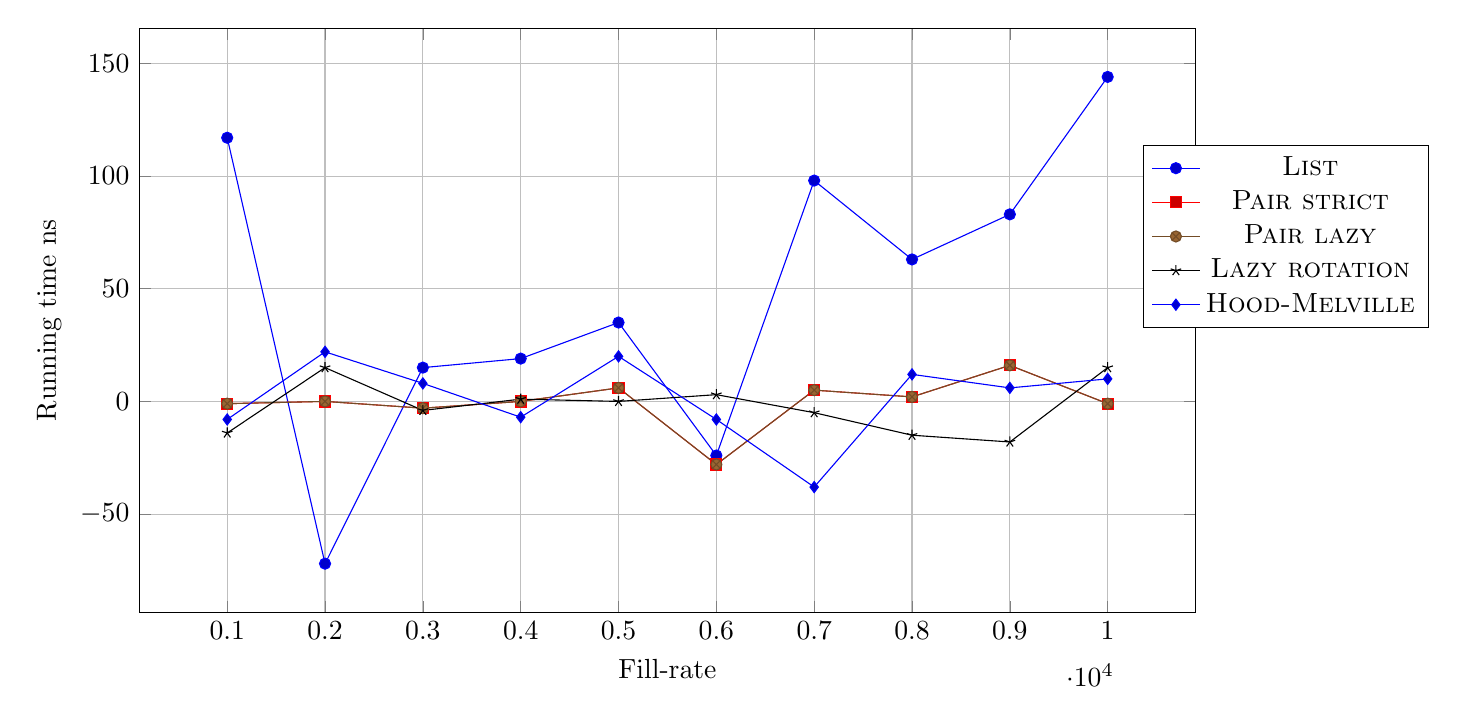
\begin{tikzpicture}
        \begin{axis}[
            xlabel = Fill-rate,
            ylabel = Running time ns,
            height=9cm,
            width=15cm,
            grid=major,
            legend style={
            at={(0.95,0.8)},
            anchor=north west}]            
            legend pos=center west
    	]
    		
    		
    	\addplot coordinates {
(1000,117)
(2000,-72)
(3000,15)
(4000,19)
(5000,35)
(6000,-24)
(7000,98)
(8000,63)
(9000,83)
(10000,144)

    	};
        
    	\addlegendentry{\textsc{List}}

                \addplot coordinates {
(1000,-1)
(2000,0)
(3000,-3)
(4000,0)
(5000,6)
(6000,-28)
(7000,5)
(8000,2)
(9000,16)
(10000,-1)

    	};
        
    	\addlegendentry{\textsc{Pair strict}}

        \addplot coordinates {
(1000,-1)
(2000,0)
(3000,-3)
(4000,0)
(5000,6)
(6000,-28)
(7000,5)
(8000,2)
(9000,16)
(10000,-1)

    	};
        
    	\addlegendentry{\textsc{Pair lazy}}

        \addplot coordinates {
(1000,-14)
(2000,15)
(3000,-4)
(4000,1)
(5000,0)
(6000,3)
(7000,-5)
(8000,-15)
(9000,-18)
(10000,15)

    	};
        
    	\addlegendentry{\textsc{Lazy rotation}}

        \addplot coordinates {
(1000,-8)
(2000,22)
(3000,8)
(4000,-7)
(5000,20)
(6000,-8)
(7000,-38)
(8000,12)
(9000,6)
(10000,10)

    	};
        
    	\addlegendentry{\textsc{Hood-Melville}}

        \end{axis}

    \end{tikzpicture}
    \captionof{figure}{TITEL}
    \label{fig:sample_figure}
\end{minipage}